%!TEX program = xelatex
\documentclass[cn,normal,black,11pt]{elegantnote}
\usepackage[T1]{fontenc}
\usepackage{wasysym}
\usepackage{multirow}

\begin{document}
\newcommand{\stunameone}{饶格奇}
\newcommand{\stunametwo}{刘雨霜}
\newcommand{\stunamethree}{}
\newcommand{\stuclassone}{2023级计算机科学与技术06班}
\newcommand{\stuclasstwo}{2023级计算机科学与技术04班}
\newcommand{\stuclassthree}{2023级计算机科学与技术04班}
\newcommand{\expname}{实验一 简单流水线与运算器实验}
\newcommand{\expdate}{2025 年 4 月 13 日}
\newcommand{\reportdate}{\number\year 年 \number\month 月 \number\day 日}
\newcommand{\exproom}{DS1410}
\newcommand{\stugrade}{优秀/良好/中等}
\newcommand{\teacher}{任骜}
% \newcommand{}{}
% \maketitle
% logo
% \centerline{
\includegraphics[width=0.25\textwidth]{logo.pdf}}

\setlist[itemize]{label=$\circ$}

\centerline{\textbf{\huge{《计算机组成原理》实验报告}}}


\begin{table}[htbp]
    \centering
    \begin{tabular}{|c|c|c|c|}
        \hline
        \multirow{3}{*}{\textbf{年级、专业、班级}} & \stuclassone & \multirow{3}{*}{\textbf{姓名}} &  \stunameone \\ &\stuclasstwo & & \stunametwo \\ &\stuclassthree & & \stunamethree\\ \hline
         \textbf{实验题目} & \multicolumn{3}{c|}{\expname} \\ 
         \hline
         \textbf{实验时间} & \expdate & \textbf{实验地点} & \exproom \\ \hline
\multirow{3}{*}{\textbf{实验成绩}} & \multirow{3}{*}{\stugrade} & \multirow{3}{*}{\textbf{实验性质}} & \Square{验证性}  \\
         &  &  &  \CheckedBox{设计性}\\
         &  &  &  \Square{综合性} \\ \hline
         \multicolumn{4}{|l|}{\textbf{教师评价:}} \\
         \multicolumn{4}{|c|}{\Square{算法/实验过程正确;}\quad \Square{源程序/实验内容提交; }\quad \Square{程序结构/实验步骤合理; } }\\
         \multicolumn{4}{|c|}{\Square{实验结果正确;}\quad\quad\quad \Square{语法、语义正确;}\quad\quad \Square{报告规范;} }\\
         \multicolumn{4}{|l|}{其他:} \\
         \multicolumn{4}{|r|}{评价教师: \teacher} \\ \hline
         \multicolumn{4}{|l|}{\textbf{实验目的}} \\
         \multicolumn{4}{|l|}{(1)掌握流水线(Pipelined)处理器的思想。} \\
         \multicolumn{4}{|l|}{(2)掌握单周期处理中执行阶段的划分。} \\
         \multicolumn{4}{|l|}{(3)了解流水线处理器遇到的冒险。} \\
         \multicolumn{4}{|l|}{(4)掌握数据前推、流水线暂停等冒险解决方式。} \\ \hline
         
    \end{tabular}
    % \caption{Caption}
    \label{tab:my_label}
\end{table}

报告完成时间: \reportdate


\newpage

\section{实验内容}
\subsection{ALU设计实验}
实验要求实现以下算术运算功能,其对应的控制码及功能如下:
\begin{table}[htbp]
    \centering
    \begin{tabular}{cccc}
        \hline
         F$_{2:0}$ & 功能 & F$_{2:0}$ & 功能  \\
         \hline
         000 & A + B(Unsigned) & 100 & $\overline{A}$ \\
         001 & A - B & \textcolor{red}{\textit{\textbf{101}}} & \textcolor{red}{\textit{\textbf{SLT}}}\\
         010 & A AND B & 110 & 未使用\\
         011 & A OR B  & 111 & 未使用\\
         \hline
    \end{tabular}
    \caption{算数运算控制码及功能}
    \label{tab:opcode}
\end{table}

\textbf{实验要求:}
\begin{enumerate}
    \item 根据ALU原理图,使用Verilog语言定义ALU模块,其中输入输出端口参考实验原理,运算指令码长度为[2:0]。
    \item 仿真时B端口输入为32h'01, A端口输入参照 4.1 中表格
    % \item 内置一个32位num2(值为32h’01)作为输入到运算器端口A;
    % \item 将sw0-sw7输入到num1,经过无符号扩展 至32位后,输入到运算器的端口B;
    % \item 运算器支持“加、减、与、或、非”5种运算,需要3位(8个操作)。将sw15-sw14输入到op作为运算器的控制信号;
    \item 实现SLT功能。
    % \item 将计算32位结果s显示到七段数码管(16进制)。
    \item 验证表\ref{tab:opcode}中所有功能。
    \item 给出RTL源程序(.v文件)
\end{enumerate}

\subsection{流水线实验}

本次实验为仿真实验,设计完成后仅需进行\textbf{行为仿真}。

\textbf{实验要求:}

% 本次实验使用Vivado的Block Memory Generator模拟数据在存储器中的存取过程。实验使用单端口ROM。初始化ROM存储器中的内容,通过开关选择相应的地址,将对应的存储器中内容读出来,并通过七段数码管显示。实验原理如图~\ref{fig:memory_experiment}所示:

% \begin{figure}[htbp]
%     \centering
%     \includegraphics[width = \textwidth]{image/1_section/memory_experiment.png}
%     \caption{Caption}
%     \label{fig:memory_experiment}
% \end{figure}

% \textbf{实验要求:}
\begin{enumerate}
    \item 实现4级流水线8bit全加器,需带有流水线暂停和刷新;
    \item 模拟流水线暂停,仿真时控制10周期后暂停流水线2周期(第2级),流水线恢复流动;
    \item 模拟流水线刷新,仿真时控制15周期时流水线刷新(第3级)。

\end{enumerate}

\section{实验设计}
\subsection{ALU}\label{sub:alu}
\subsubsection{功能描述}
该 ALU 实现加法、减法、按位与、按位或、取反及无符号小于判断等基础运算功能,支持 8 位
与 32 位输入,输出 32 位结果,并在数码管上进行显示。
\subsubsection{接口定义}
\begin{table}[htp]
\caption{接口定义}\label{tab:signaldef}
\begin{center}
	\begin{tabular}{|l|l|l|p{6cm}|}
	\hline
	\textbf{信号名} & \textbf{方向} & \textbf{位宽} & \textbf{功能描述}\\ \hline \hline
	num1	&Input	&8-bit	&操作数1\\
	num2	&Input	&32-bits	& 操作数2\\
	op	&Output	&3-bits	& 操作码\\
	result	&Output	&32-bits & 计算结果\\
	seg &Output &7-bits & 七段数码管\\
	clk &Input &1-bit & 时钟信号\\
	reset &Input &1-bit & 复位信号\\
	\hline
	\end{tabular}
\end{center}
\end{table}

\subsubsection{逻辑控制}
本 ALU 模块采用组合逻辑控制方式,不使用时序触发的有限状态机(FSM)。由于 ALU 
运算为即时反应型逻辑(无时序依赖),其控制流程可简化为单周期组合逻辑响应,无需状态跳转。
模块通过将 8 位输入零扩展为 32 位,并根据 3 位操作码执行加、减、与、或、取反和小于判断等运算,非法操作码输出全 x。
ALU的控制逻辑使用组合逻辑电路实现,具体如下:
\begin{figure}[htbp]
    \centering
    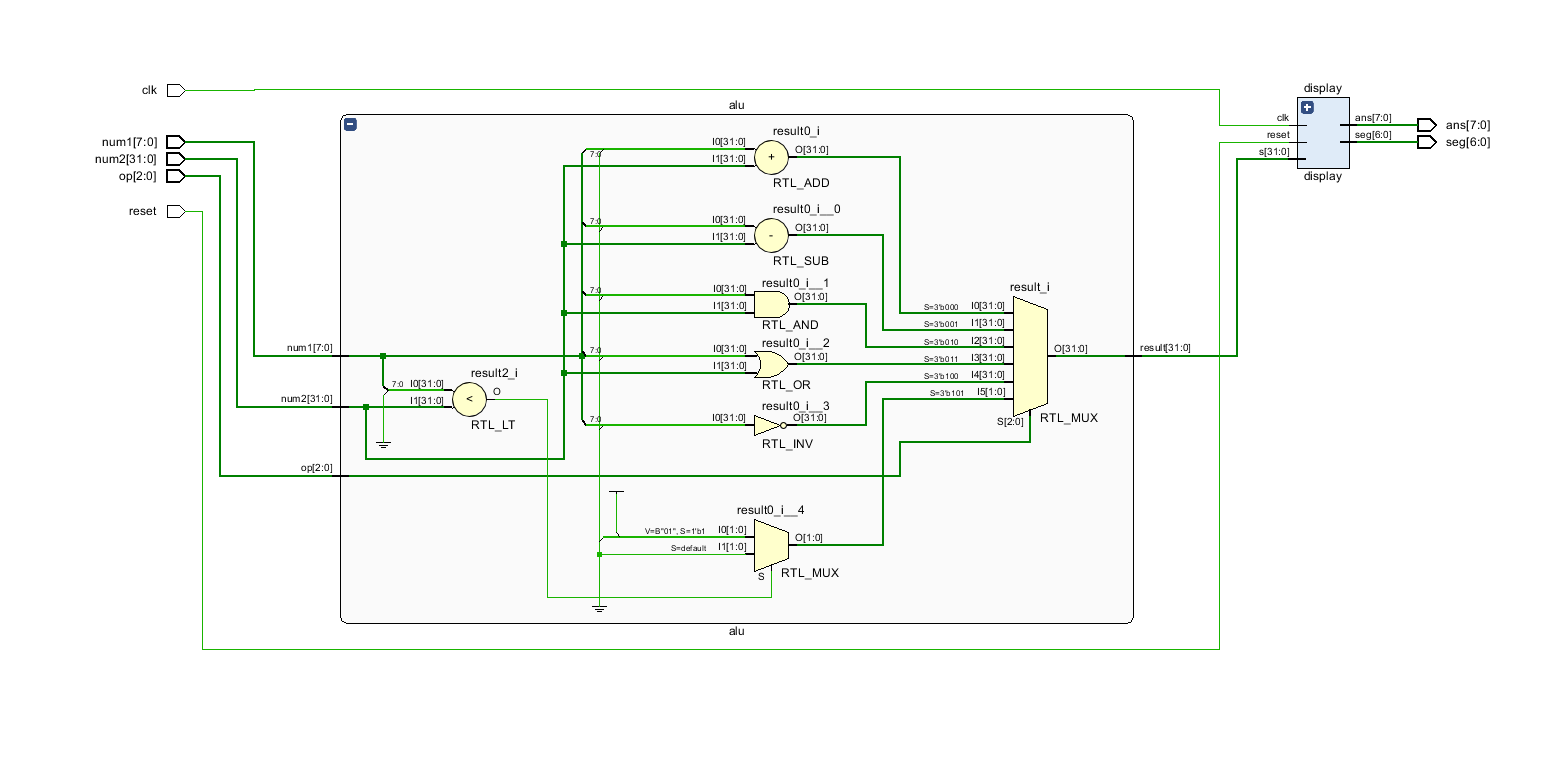
\includegraphics[width=0.7\textwidth]{image/yingjian.png}
    \caption{ALU控制逻辑电路}
	\label{fig:alu_control}
\end{figure}
\subsection{有阻塞4级8bit全加器}\label{sub:ctl}
\subsubsection{功能描述}
本模块 \texttt{adder} 是一个采用四级流水线结构实现的 32 位加法器。模块接收两个 32 位输入操作数 \texttt{num1} 和 \texttt{num2},通过每阶段处理 8 位数据逐步完成加法,并支持输入初始进位 \texttt{cin}。模块支持异步复位 \texttt{reset},每级流水线的刷新控制 \texttt{refresh} 以及暂停控制 \texttt{stop},并提供各阶段调试输出与流水线状态指示。最终输出结果为 32 位加法结果 \texttt{ans} 和最终进位 \texttt{cout}。

\subsubsection{接口定义}
\text{}见下表
\begin{table}[htp]
	\caption{adder 模块接口定义}\label{tab:adder_interface}
	\begin{center}
		\begin{tabular}{|l|l|l|p{6cm}|}
		\hline
		\textbf{信号名} & \textbf{方向} & \textbf{位宽} & \textbf{功能描述} \\ \hline \hline
		clk             & Input  & 1     & 时钟信号,驱动流水线各阶段时序逻辑 \\
		reset           & Input  & 1     & 异步复位信号,高电平有效,清除所有状态 \\
	refresh         & Input  & 4     & 各流水线级刷新信号,高电平有效清除对应阶段状态 \\
	stop            & Input  & 4     & 各流水线级暂停信号,高电平阻止流水前传 \\
	cin             & Input  & 1     & 初始加法进位 \\
	validin         & Input  & 1     & 输入数据有效标志 \\
	out\_allow      & Input  & 1     & 输出允许信号,决定是否将结果输出 \\
	num1            & Input  & 32    & 加法器第一个操作数 \\
	num2            & Input  & 32    & 加法器第二个操作数 \\
	validout        & Output & 1     & 输出数据有效标志,表示结果已准备好 \\
	ans             & Output & 32    & 最终加法结果 \\
	cout            & Output & 1     & 最终进位输出 \\
	debug\_sum1     & Output & 8     & 第一阶段的部分加法结果(用于Debug) \\
	debug\_sum2     & Output & 16    & 第二阶段的部分加法结果(用于Debug) \\
	debug\_sum3     & Output & 24    & 第三阶段的部分加法结果(用于Debug) \\
	debug\_sum4     & Output & 32    & 第四阶段(最终)的加法结果(用于Debug) \\
	pipe1\_valid\_out & Output & 1    & 第一阶段有效状态指示 \\
	pipe2\_valid\_out & Output & 1    & 第二阶段有效状态指示 \\
	pipe3\_valid\_out & Output & 1    & 第三阶段有效状态指示 \\
	pipe4\_valid\_out & Output & 1    & 第四阶段有效状态指示 \\
		\hline
		\end{tabular}
	\end{center}
	\end{table}
\subsubsection{逻辑控制}

本模块采用四级流水线结构,逐步完成 32 位加法操作,每级处理 8 位数据,并传递进位信息,详细逻辑如下:

\begin{itemize}
    \item \textbf{流水线允许控制}:每一级通过 \texttt{allowin} 信号判断是否能接收数据,条件为本级未被 \texttt{stop[i]} 阻塞,且下一级允许传输数据,或本级当前无效。
    
    \item \textbf{数据传递与寄存}:每一阶段使用寄存器保存当前级别的部分和与操作数剩余高位,下一阶段继续处理更高位加法并拼接形成完整结果。
    
    \item \textbf{进位传递逻辑}:初始进位 \texttt{cin} 输入到第一阶段,后续每级进位通过前一级的进位累加传递。
    
    \item \textbf{复位与刷新机制}:模块支持复位信号 \texttt{reset},用于清除所有阶段的 \texttt{valid} 状态。单独阶段可通过对应的 \texttt{refresh[i]} 控制信号进行刷新清除。
    
    \item \textbf{输出控制}:最终输出由第四级流水线完成,其输出受 \texttt{out\_allow} 控制。若该阶段有效且输出允许,则输出 \texttt{ans} 和 \texttt{cout},同时置 \texttt{validout} 为高。
    
    \item \textbf{调试输出}:模块提供每一级流水的调试输出 \texttt{debug\_sum*},用于观察中间和的变化情况,辅助调试与验证。
\end{itemize}


\section{实验过程记录}
\subsection{问题1:仿真多数据出现不定态X}
\textbf{问题描述:}refile的内部信号未初始化0,加之controller中的控制信号在某些情况规定为x,虽然逻辑上在某些情况这些控制信号是0是1都是可以的,
但是会影响到其他运算,导致不定态在运算中不断传递。

\textbf{解决方案:}将controller中的控制信号为x改成0。
\subsection{问题2:ALU无法读到数据}
\textbf{问题描述:}$or$ 指令无法读到 $addi \$2, \$0, 5$ 的数据,导致 $\$4$ 的值错误。因为regfile中 \$2的数据输入与读取在同一上升沿,故无法取到正确的数。

\textbf{解决方案:}将regfile的 $posedge clk$ 改为 $negedge clk $,使得数据提前半周期读入regfile。
\subsection{问题3:datamemory最后无法正确输出已经存入的值}
\textbf{问题描述:}通过仿真发现datamemory的输出延后实际信号memwriteM三周期。

\textbf{解决方案:}通过排查发现接口接错导致memwriteM没有正确输出,而是将memwriteE当作memwriteM输出。于是将输出接口修正。

\section{实验结果及分析}
\begin{figure}[H]
    \centering
    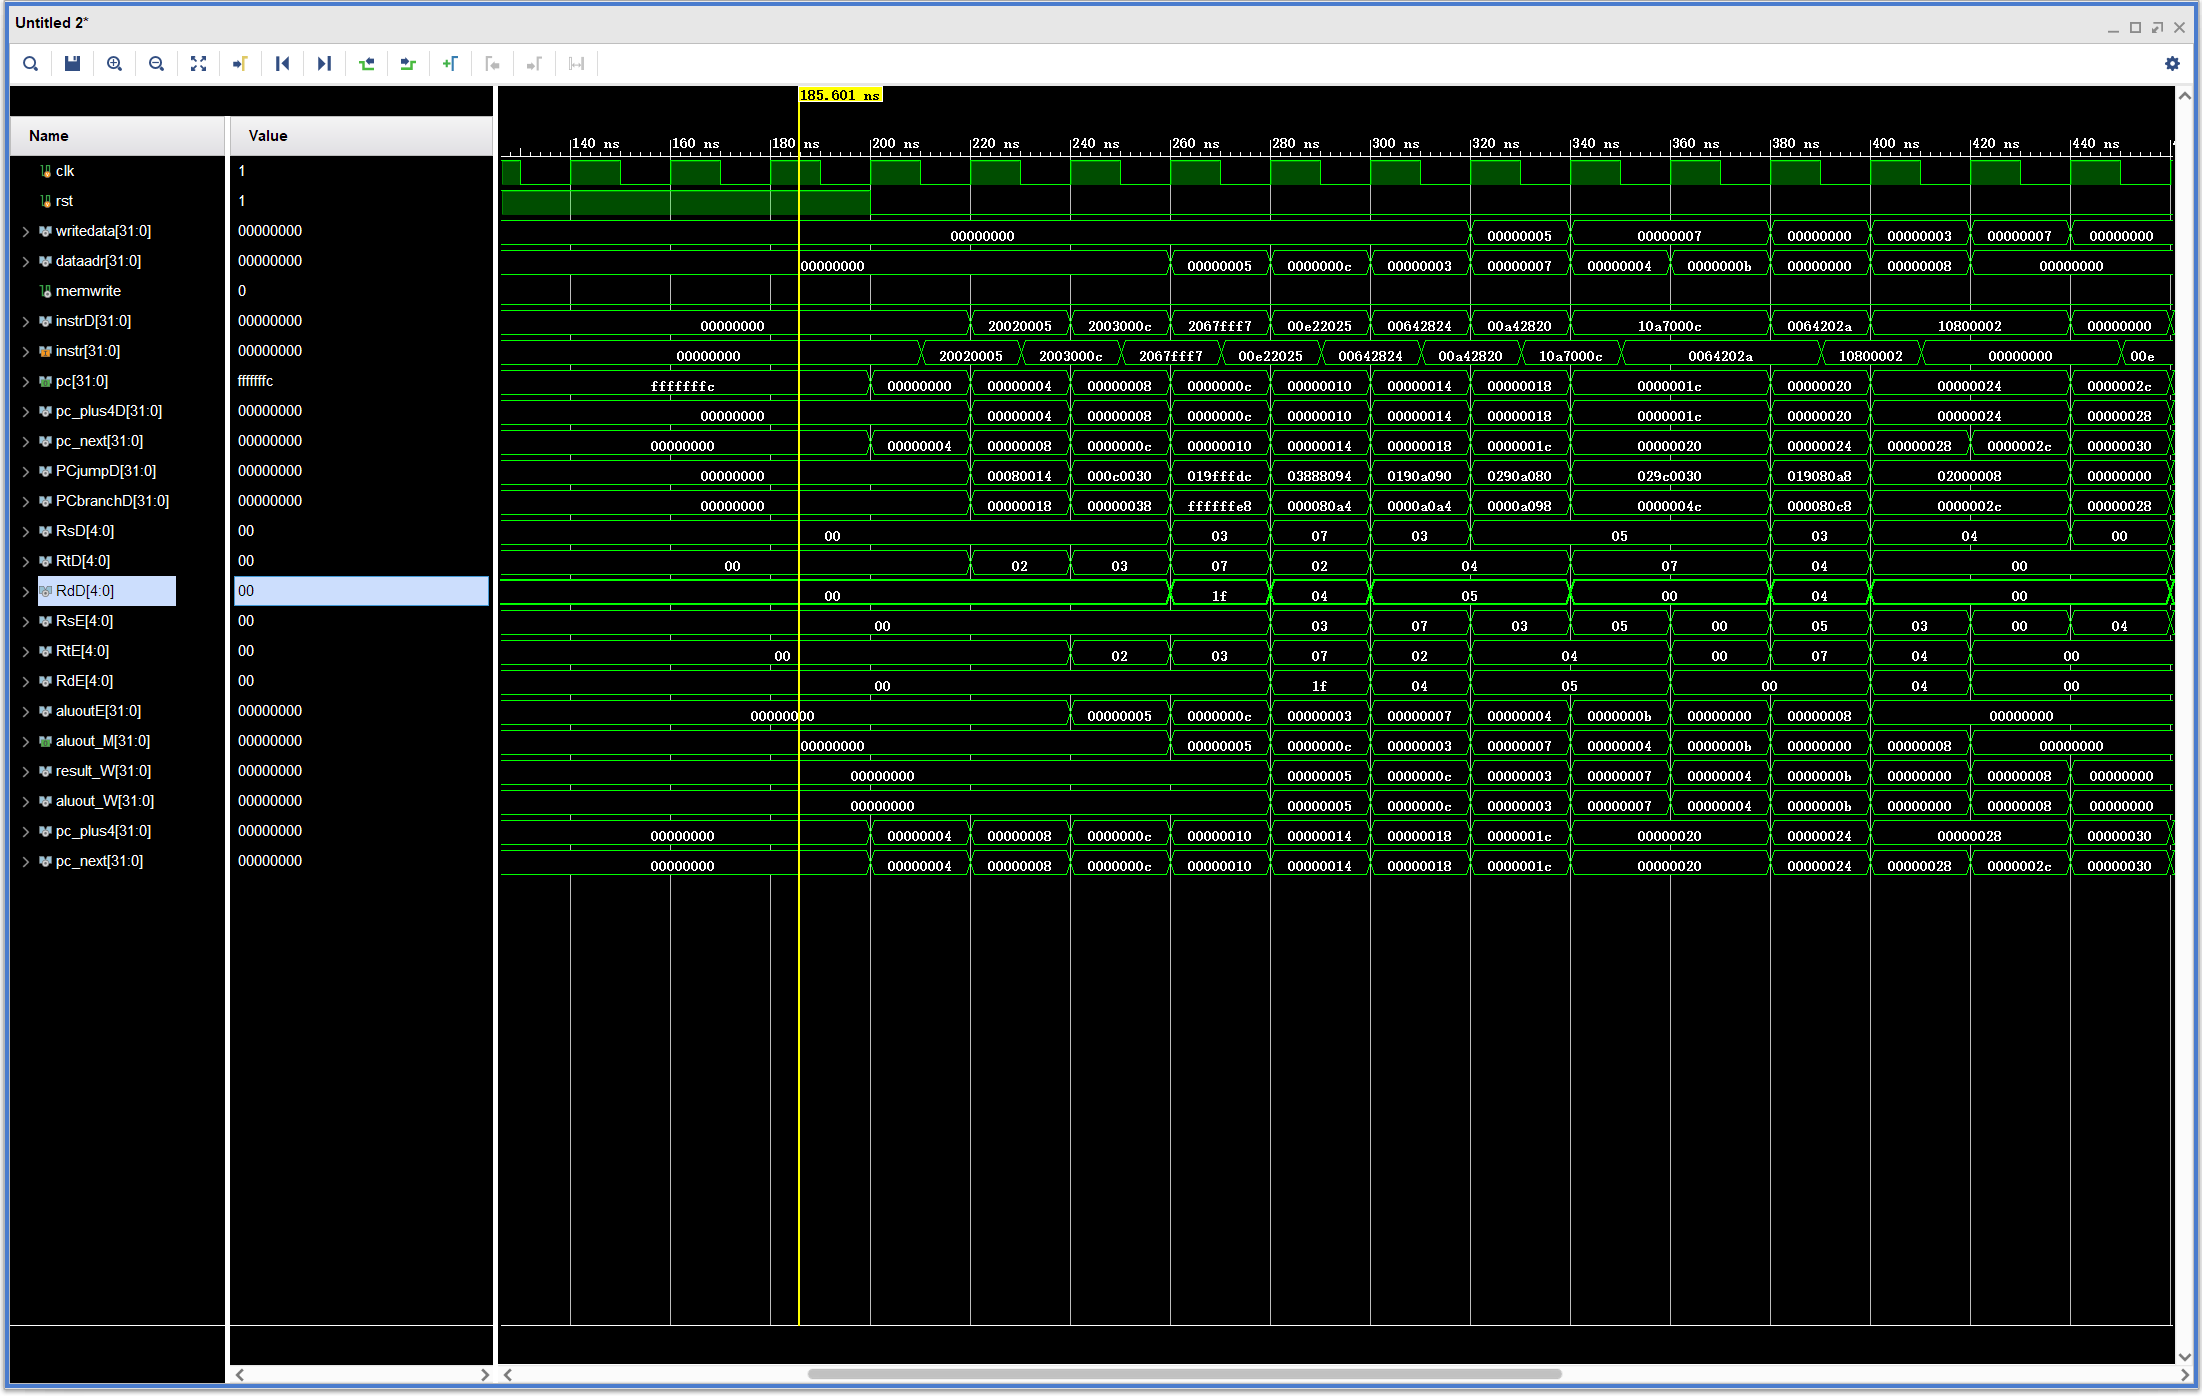
\includegraphics[width=0.9\textwidth]{image/sim1.png}
    \caption{仿真结果1}
    \label{fig:sim1}
\end{figure}
\begin{figure}[H]
    \centering
    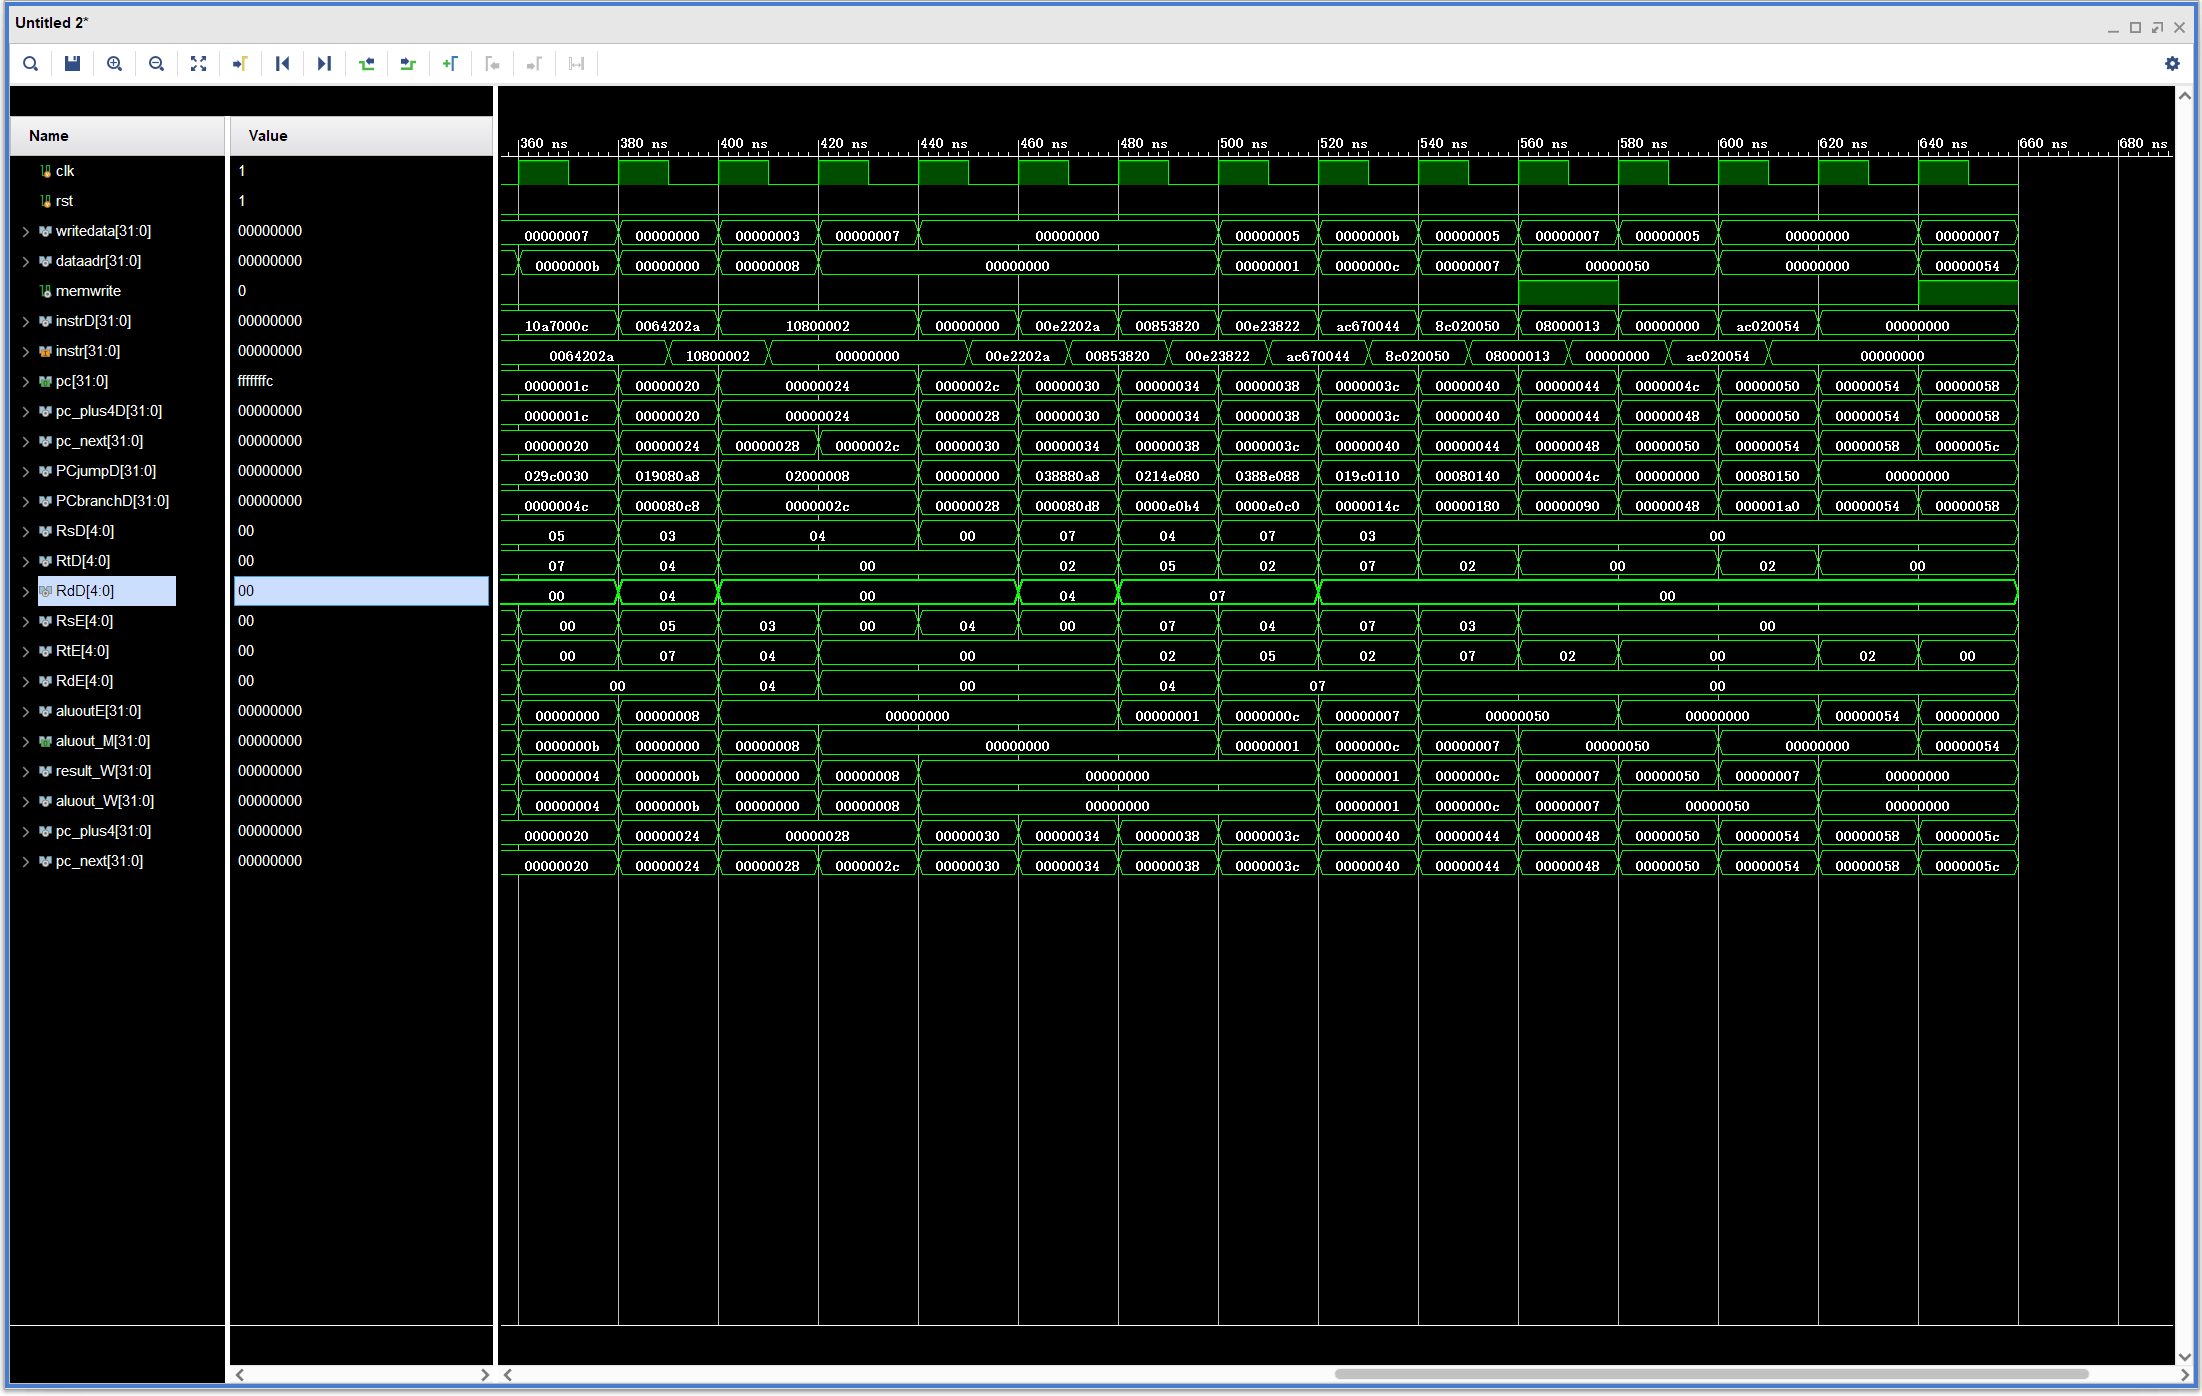
\includegraphics[width=0.9\textwidth]{image/sim2.png}
    \caption{仿真结果2}
    \label{fig:sim2}
\end{figure}
\begin{figure}[H]
    \centering
    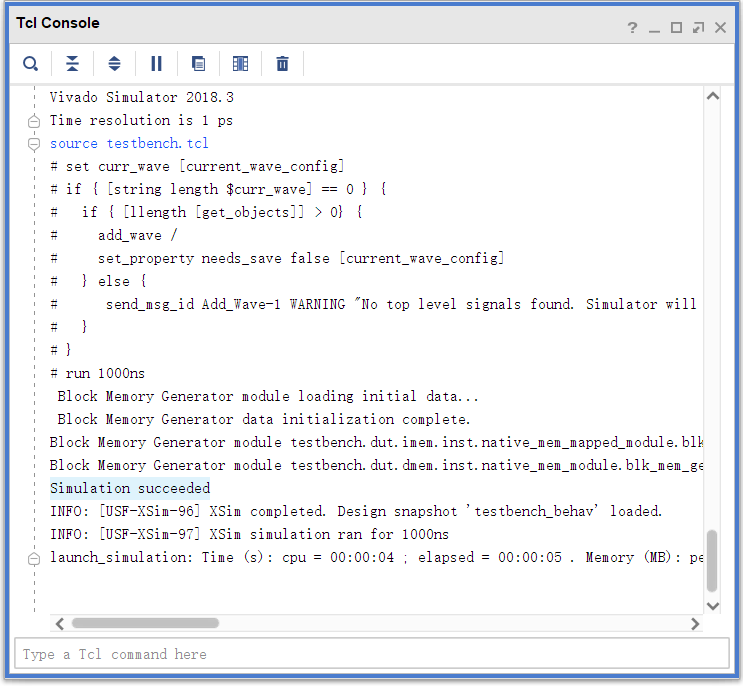
\includegraphics[width=0.9\textwidth]{image/tcl.png}
    \caption{Simulation succeeded}
    \label{fig:tcl}
\end{figure}

\appendix
\section{Controller代码}
\textcolor{red}{仅需要根据需要,在一个模块完成控制器的,直接填写,多个模块(maindec、aludec)分别加入新的lstlisting并填写(红字为内容说明,请删除)}
\begin{lstlisting}[language=Verilog]

\end{lstlisting}


\end{document}
